%Version 2.1 April 2023
% See section 11 of the User Manual for version history
%
%%%%%%%%%%%%%%%%%%%%%%%%%%%%%%%%%%%%%%%%%%%%%%%%%%%%%%%%%%%%%%%%%%%%%%
%%                                                                 %%
%% Please do not use \input{...} to include other tex files.       %%
%% Submit your LaTeX manuscript as one .tex document.              %%
%%                                                                 %%
%% All additional figures and files should be attached             %%
%% separately and not embedded in the \TeX\ document itself.       %%
%%                                                                 %%
%%%%%%%%%%%%%%%%%%%%%%%%%%%%%%%%%%%%%%%%%%%%%%%%%%%%%%%%%%%%%%%%%%%%%

%%\documentclass[referee,sn-basic]{sn-jnl}% referee option is meant for double line spacing

%%\documentclass[lineno,sn-basic]{sn-jnl}% Basic Springer Nature Reference Style/Chemistry Reference Style

%%\documentclass[pdflatex,sn-basic]{sn-jnl}% Basic Springer Nature Reference 
 
\documentclass[pdflatex, sn-nature]{sn-jnl}% Style for submissions to Nature Portfolio 

%%%% Standard Packages
\usepackage{graphicx}%
\usepackage{multirow}%
\usepackage{amsmath,amssymb,amsfonts}%
\usepackage{amsthm}%
\usepackage{mathrsfs}%
\usepackage[title]{appendix}%
\usepackage{xcolor}%
\usepackage{textcomp}%
\usepackage{manyfoot}%
\usepackage{booktabs}%
\usepackage{algorithm}%
\usepackage{algorithmicx}%
\usepackage{algpseudocode}%
\usepackage{listings}%
\usepackage{gensymb} %added by V. Van der Meersch
\usepackage{comment} %added by V. Van der Meersch
 \usepackage{textcomp} %added by V. Van der Meersch
 \newcommand{\textappr}{\raisebox{0.5ex}{\texttildelow}} %added by V. Van der Meersch

%%%%

%%%%%=============================================================================%%%%
%%%%  Remarks: This template is provided to aid authors with the preparation
%%%%  of original research articles intended for submission to journals published 
%%%%  by Springer Nature. The guidance has been prepared in partnership with 
%%%%  production teams to conform to Springer Nature technical requirements. 
%%%%  Editorial and presentation requirements differ among journal portfolios and 
%%%%  research disciplines. You may find sections in this template are irrelevant 
%%%%  to your work and are empowered to omit any such section if allowed by the 
%%%%  journal you intend to submit to. The submission guidelines and policies 
%%%%  of the journal take precedence. A detailed User Manual is available in the 
%%%%  template package for technical guidance.
%%%%%=============================================================================%%%%

%\jyear{2021}%

\raggedbottom
\unnumbered% uncomment this for unnumbered level heads

\begin{document}

\title[Article Title]{Temporary titles: Causal relationships ensure model robustness  / Causal relationships improve model projections reliability / Improving forecasting with process-based modeling}

\author*[1]{\fnm{Victor} \sur{Van der Meersch}}\email{victor.vandermeersch@cefe.cnrs.fr}
\author[2]{\fnm{Edward} \sur{Armstrong}}
\author[1]{\fnm{Florent} \sur{Mouillot}}
\author[3]{\fnm{Anne} \sur{Duputié}}
\author[4]{\fnm{Cristophe} \sur{Randin}}
\author[5]{\fnm{Hendrik} \sur{Davi}}
\author[6]{\fnm{Frédérik} \sur{Saltré}}
\author[1]{\fnm{Isabelle} \sur{Chuine}}

\affil[1]{\orgdiv{CEFE}, \orgname{Université de Montpellier, CNRS, EPHE, IRD}, \orgaddress{\city{Montpellier}, \country{France}}}
\affil[2]{\orgdiv{Dept. of Geosciences and Geography}, \orgname{University of Helsinki}, \orgaddress{\city{Helsinki}, \country{Finland}}}
\affil[3]{\orgdiv{UMR 8198-EEP-Evo-Eco-Paleo}, \orgname{Université de Lille, CNRS}, \orgaddress{\city{Lille}, \country{France}}}
\affil[4]{\orgdiv{Dept. of Ecology and Evolution}, \orgname{Univ. Lausanne}, \orgaddress{\city{Lausanne}, \country{Switzerland}}}
\affil[5]{\orgdiv{URFM}, \orgname{INRAE}, \orgaddress{\city{Avignon}, \country{France}}}
\affil[6]{\orgdiv{Global Ecology}, \orgname{College of Science and Engineering, Flinders University}, \orgaddress{\city{Adelaide}, \country{Australia}}}

\abstract{The recent acceleration of global climate warming has increased the need for reliable  ecological forecasts, especially for species distributions, which are widely used by natural resources managers. Such forecasts, however, are produced with varied modeling approaches with little information on which perform well given the novel climatic conditions expected with continued anthropogenic greenhouse gas emission. Here, we leverage the most recent period of climate novelty---the early Holocene---to compare the performance of  correlative models (CSDMs), and two versions of process-based models (PBMs) differing in their calibration method. We hindcast the range shift of five tree species across Europe over the last 12,000 years, taking into account migration, and evaluate their predictions against fossil pollen records. While projections of all models are less reliable moving back to the past, we show that the  performance of correlative models decreases \textappr2.5 times faster than that of process-based models when climatic dissimilarity rises. We further find that inverse calibration of PBMs, using the same data as CSDMs, does not affect their reliability. These findings highlight the importance of considering mechanisms to ensure model robustness, and provide a promising framework to promote process-based approaches to deliver more accurate projections in the future.}

\keywords{Species range shift, ecological modelling, model transferability, tree species}

\maketitle

\newpage

% CUTE BABY: we need reliable projections of the distribution of species

% WEREWOLF: models perform less well under different conditions than those in which they were built/calibrated... and in addition, in the future, climatic conditions are expected to be very different
% And we don't know which model will be the most robust! :-( 

% SILVER BULLET: through this comparison in the Holocene, we highlight that it is necessary to model cause-and-effect relationships describing the abilities of species to survive/grow/reproduce in various env conditions
% and that inverse calibration using large-scale data may serve as an important step to facilitate the use of process-based models in a very near future :-) :-) :-) yippee!

\section{Main}
%emw13Jan -- you say 'modellers' below but for NCC I would keep the focus really broad -- you want this to clearly matter to managers, climatologists, modellers, ecologists etc.. I think here you could set up more how important SDMs are first.   
Modelling is key to understanding how climate change will impact ecosystems and biogeochemical cycles. As the demand for reliable projections of nature contribution to people is increasing, thorough evaluations of ecological model performances should be a major focus to provide credible information to natural resource managers, decision makers and stakeholders \cite{Dawson2011, Mouquet2015, Pacifici2015}.

%emw13Jan -- I liked the below, but I wanted to sound a little more important and exciting.
One approach to evaluate model reliability is to compare their predictions to observations from previous time periods, i.e. hindcasting. Hindcasting can indeed inform whether models capture, implicitly or explicitly, the essential processes required to provide reliable projections in conditions significantly different from the present. By looking far in the past, paleo-archives have proven to offer a unique opportunity to understand long-term both climate and biodiversity dynamics \cite{Fordham2020} and to test model robustness and transferability (model capacity to maintain its performance in changing conditions \cite{UribeRivera2022})   \cite{Braconnot2012, Maguire2015}.  So far, models have often failed to predict accurately species distribution and biospheric components \cite{Veloz2012, Pearman2008, Roberts2012, Foley2013, Maguire2016}, when being compared to paleoclimate reconstructions and fossil records. Interpreting their projections in climatic conditions that differ significantly from the present, such as future no-analogue climatic conditions \cite{Williams2007}, becomes challenging because the guarantee that model forecasts for the 21\textsuperscript{st} century will be reliable is small \cite{Fitzpatrick2018}.

%emw13Jan -- depending on when you introduce the Holocene, you could insert a quick review of it in a sentence, something like 'the period after the last glacial, which began with abrupt climate change (immortalized now in Marvel films) followed by a long period of climatic stability (maybe: during which much of human culture etc. developed) that was mostly uninterrupted until recent anthropogenic warming. 
While exact matches to expected 21\textsuperscript{st}-century climatic conditions do not exist in historical records \cite{Burke2018}, the dissimilarity between 20\textsuperscript{th} and 21\textsuperscript{st} century median climatic conditions (\hyperref[methods]{Methods}) falls within the range of dissimilarity encountered since the beginning of the Holocene (12,000 years Before Present, hereafter 1000 year Before Present = kyr BP, \hyperref[climatic_dissimilarity]{Fig. 1}). This period takes place after the Last Glacial Maximum (26.5-19 kyrs BP) and began with an abrupt climate warming followed by a long, almost uninterrupted, period of climatic stability until recent anthropogenic warming (Extended Data Fig. 1).  

\begin{figure}[ht]
\centering
\hspace*{-0.6in}
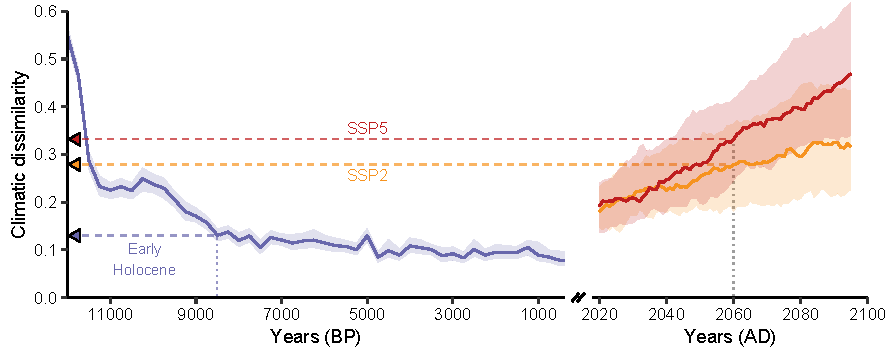
\includegraphics[scale=1]{climatic_dissimilarity.pdf}
%emw13Jan -- I really like this figure! Can you label the dashed lines (SSP..) directly on the figure?
\caption{\textbf{Evolution of climatic dissimilarity under past (12k-500 yr BP) and future (2005-2100) climate changes, relative to 1901-2000}. Climatic dissimilarity is computed as 1-Sørensen similarity between bootstrapped climatic hypervolumes. Lines represent median dissimilarity, shaded areas represent 90\% confidence intervals. Blue corresponds to paleoclimate based on HadCM3B model. Yellow and red correspond to SSP245 and SSP585 scenarios, each based on 30 models. Blue triangle on y-axis indicates the limit between Early Holocene (before 8200BP) and Late-Middle Holocene (after 8200BP). Yellow and red triangles indicate the expected level of climatic dissimilarity in 2060 for SSP245 and SSP585 scenarios. Note that the x-axis scale changes across past and future panels.}\label{climatic_dissimilarity}
\end{figure}

Species distribution modeling (SDM) is a powerful tool for projecting species geographical distribution as a function of environmental data (e.g., mean annual temperature, mean annual precipitation). Most studies have focused on correlative models (CSDMs, also called environmental niche models), which infer statistical relationships between observations of species occurrences and environmental predictors \cite{Dormann2012}. Their high flexibility and low computational complexity make them by far the most widely used tool for deciding on species conservation plans and policy regimes. However, under novel climate conditions, new unobserved portions of a species’ ecological niche may appear, which are not captured by these correlative approaches. For example, when challenged with distant past climates, CSDM predictive performance appeared to drop significantly \cite{Maguire2016}, which questions their ability to provide reliable projections in the future \cite{Fitzpatrick2018}. Alternative approach to CSDMs are process-based models (PBMs) that rely on explicit formulations of the mechanisms driving the distribution of a given species (e.g., physiological, ecological and demographic processes). They come from decades of experiments and observations, including extreme conditions in laboratory \cite{Seehausen2017}, and climate manipulations such as CO2 enrichment \cite{Jiang2020} or rainfall exclusion \cite{Gavinet2019}. Because these models are not based on a statistical relationship between present-day species occurrences (presence/absence) and environmental variables, they are expected to provide better predictions of species responses to climate change  \cite{Evans2012, Singer2016}. However, their reliability depends on our level of understanding of how ecophysiological processes are affected by environmental conditions, and the availability of large amount of observations and measurements to calibrate their many parameters  \cite{Evans2016}. Where data is lacking, inverse calibration using large-scale data can still help to calibrate fitted PBMs \cite{Dormann2012, VanderMeersch2023}. PBMs often make more conservative projections in future climates than those of CSDMs which predict larger changes \cite{Morin2009, Cheaib2012, Gritti2013}, and there is still a debate on which approach might be the most reliable.

%emw13Jan -- I think this needs to perhaps be its own paragraph? And be much stronger -- make it clear that we have a problem (werewolf) that you will solve (kill). 
Despite the growing interest for PBMs in predictive ecology \cite{Connolly2017, Urban2016, Pilowsky2022}, the common belief that they should provide more reliable projections of future species range shifts has never been verified as well as the reasons why they could do so. Very few studies have indeed gone beyond qualitative comparisons between CSDMs and PBMs and compared thoroughly their performance. This has been done for example using virtual species \cite{Zurell2016}, exotic species in native and newly colonized areas \cite{Higgins2020}, or in the recent past \cite{Fordham2018}. While PBMs have shown their usefulness for paleoecological studies \cite{Saltre2013, Ruosch2016, Schwoerer2014}, the extent to which they can provide more reliable predictions than CSDMs in the far past remains unknown \cite{UribeRivera2022, Briscoe2019}. Such assessment is now a top priority to guide more efficiently biodiversity and ecosystems management plans \cite{Pacifici2015}, but also to improve biosphere/atmosphere interaction models.

%emw13Jan -- 'shortcomings' sounds to me like a small problem; need something more like: gap, problem, critical challenge ... and make sure you have built up to it. 
Here, we address this critical gap by using multiple CSDMs and PBMs, combined with a migration model, to simulate paleodistributions of five emblematic tree species of Europe at a high-temporal resolution since 12 kyr BP. We assess first whether CSDMs or PBMs predict best species paleodistributions, and second whether model performance is related to their hypotheses (relationships describing explicit biological mechanisms or not) or their calibration methods. To do so, we compared three types of models: CSDMs, PBMs and PBMs calibrated in the same way as CSDMs (inverse calibration using species occurrence data and a novel type of algorithm, \hyperref[methods]{Methods} and \citep{VanderMeersch2023}). 
%/////// J'ENLEVERAIS CE QUI SUIT//////Our targeted models predict species potential distribution based solely on climatic and soil conditions. However, species migration %could have been a more limiting factor than climate during tree post-glacial expansion \cite{Saltre2013}, and could also prevent trees to track future climate changes. %Thus, to provide more accurate dynamic predictions of species distributions and compare them to pollen paleorecords, we simulated tree migration as well. Encompassing the %entire spectrum of models, from correlative models to process-based models and their hybrid data-driven counterparts, allowed us identifying the key features necessary for %building robust models. 

%emw13Jan -- I would separate out the sentence below from the above so you have a clear, short statement of the problem and how you address it. You can probably fit the below sentence into results & discussion
% We additionally quantified the dissimilarity between past climatic conditions and historical conditions (in terms of hypervolume overlap, \hyperref[methods]{Methods}) to investigate its effects on model performance.
The maximum level of climatic dissimilarity for which we evaluated model performance corresponds to the level that should be reached by the end of the century according to SSP2, and by the middle of the century according to SSP5.  We find that the predictive performance of all models decreased moving back in time and in increasingly novel climates, but PBMs overall maintained a better performance and a higher transferability in distant climatic conditions than CSDMs. We also find that inverse calibration does not alter significantly PBMs performance and long-term transferability.  First, this result suggests that PBMs robustness is convey by the biological mechanisms they describe rather than their methods of calibration. Second, this result highlights a promising method to calibrate PBMs which could offer an avenue for their development which has been drastically slowed down by the availability of data to calibrate them.

\begin{figure}
\centering
\vspace*{-0.6in}
\hspace*{-0.35in}
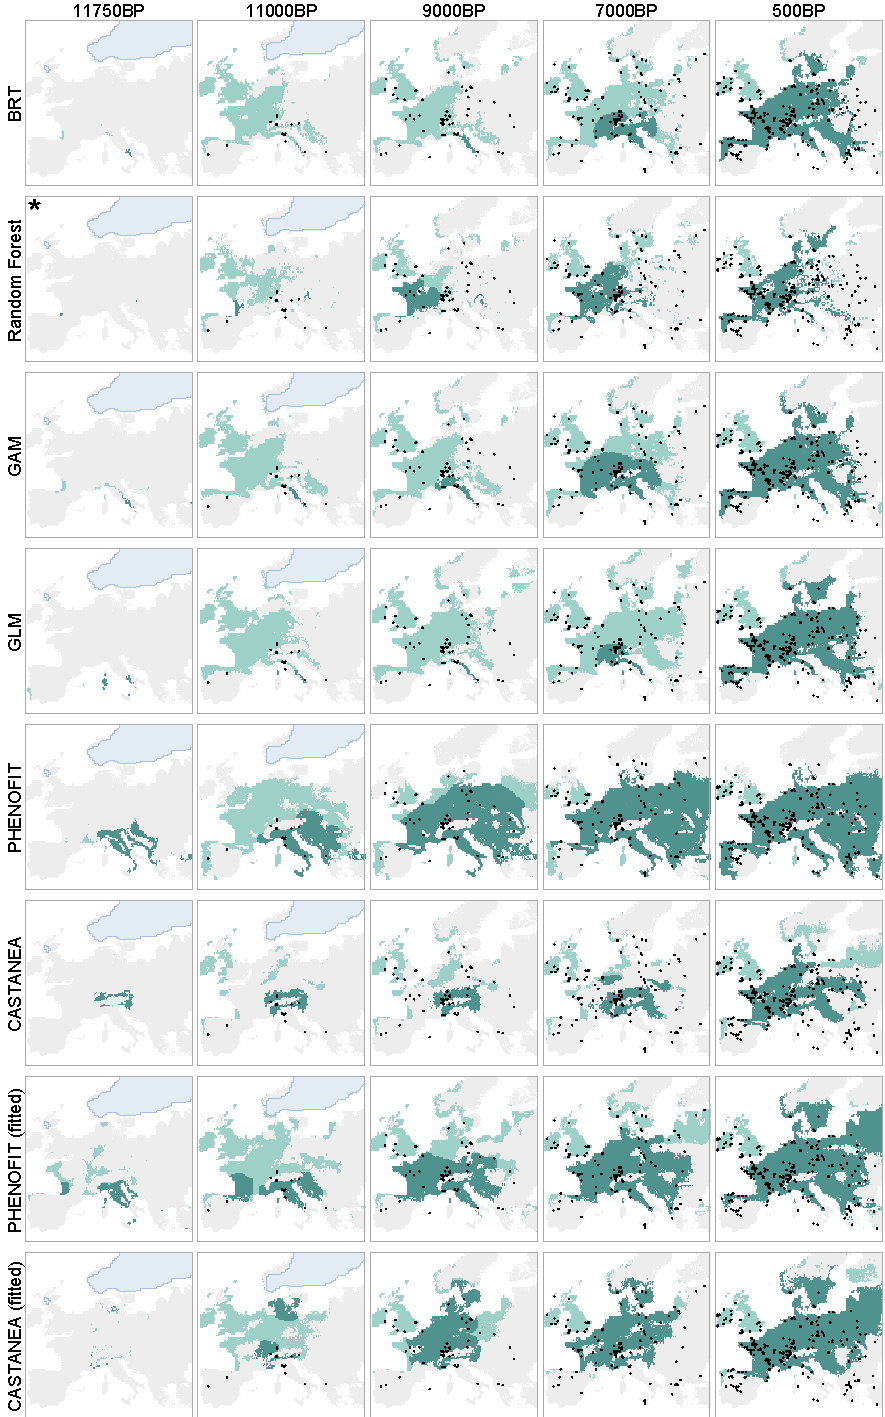
\includegraphics[scale=0.95]{quercus_deciduous_simulations.pdf}
\caption{\textbf{Example of paleosimulations obtained with the eight models used in this study for deciduous oaks.} Four first rows correspond to the four correlative models (boosted regression tree, down-sampled random forest, generalized additive model, generalized linear model with lasso regularization). Four last rows correspond to two different versions (expert calibration and inverse calibration) of two process-based models (PHENOFIT and CASTANEA). Light green area is the modelled suitable area, dark green area is the colonized area (after migration). Light blue represents the ice sheet extent. Black dots are deciduous oak fossil pollen occurrences. Model for which migration started at 117500 BP rather than 12000 BP is marked with an asterisk. "BP" stands for "before present" (1950).}\label{quercus_migration}
\end{figure}



\renewcommand\labelitemi{{\boldmath$\cdot$}}
\begin{itemize}
\setlength\itemsep{1em}
\item \emph{Models hindcast skills}\par
\item As observed in previous long term historical assessments, all models showed a decrease of their performance by moving further away in the past, in more different climatic conditions (\hyperref[past_performance]{Fig. 3a}).
%emw13Jan -- whhy not use \ref{fig:past_performance} to directly label your figure number?
Without migration, CSDMs and PBMs' abilities to predict fossil pollen occurrence were similar (Extended Data Fig. 11), with an average Sørensen index decrease of $-0.209\pm0.0210$ (paired Wilcoxon-test, $P<0.0001$) and TSS decrease of $-0.145\pm0.0424$ (paired Wilcoxon-test, $P=0.00016$) between Late-Middle Holocene (> 8,200BP) and Early Holocene (< 8,200BP).  When accounting for migration since 12,000BP, novel climatic conditions led to a stronger decrease in the predictive performance of CSDMs (slope of Beta regression, $-10.97$, 95\% CI $[-13.4, -8.63]$) than those of fitted PBMs ($-6.14$, 95\% CI $[-8.93, -3.46]$) and expert PBMs ($-4.47$, 95\% CI $[-7.16, -1.90]$). CSDMs and fitted PBMs were significantly better at predicting tree distribution in the near past (Late-Middle Holocene) than expert PBMs (pairwise Conover-Iman tests, respectively $P=0.035$ and $P=0.0029$, \hyperref[past_performance]{Fig. 3c}), indicating their closer fit to current species distributions, whereas both expert and fitted PBMs performed better than CSDMs in the Early Holocene (pairwise Conover-Iman tests, both $P<0.0001$, \hyperref[past_performance]{Fig. 3c}). 
Expert and fitted PBMs show no significant differences in their performance and transferability although expert PBMs shows slightly higher transferability  (\hyperref[past_performance]{Fig. 3b}). Expert and fitted PBMs are thus less affected by the increase in climatic dissimilarity, where species-climate relationships built in CSDMs may not hold true. %emw13Jan -- (below) work in some of these predictions/expectations to the intro?
This shows that PBMs higher transferability is rather conveyed by the mechanisms represented in the models than their method of calibration. Thus, in addition to allowing separate investigation of the effects of environmental stresses on tree survival, growth, and reproduction, biological mechanisms represented in PBMs are thus critical to ensure higher model robustness in more novel climatic conditions. This is an important and new result which both argues for a wider use of PBMs to provide forecasts of biodiversity and ecosystems distributions in the future and opens a new avenue  to reach this goal by using inverse modelling technics to calibrate them. 
\item Models performances were not stable across species, and exhibited both similarities and differences across time (Extended Data Fig. 10). More specifically, models exhibited the same overall performance decrease against \emph{Fagus} pollen records, whereas CSDM performance decline was substantially faster than expert and fitted PBMs for deciduous \emph{Quercus}. All models show low predictive power regarding evergreen \emph{Quercus} distribution even in the recent past compared to other species, especially CSDMs which failed to predict its presence along the Atlantic coast (Extended Data Fig. 7).

\item Most of the variability among models performance is due to the differences in their projections during the late Pleistocene-Early Holocene (xxx). This period  corresponds to a global deglaciation which lasted for a few centuries and occurred after the cooling of the Younger Dryas interval  (xxxx, Extended Data Fig. 1). This rapid warming episode explains the rapid decrease of climatic dissimilarity to present between 12 kyr BP and 11 kyr BP (\hyperref[climatic_dissimilarity]{Fig. 1}). Since the migration model is identical across all simulations, differences of performance between models across the Holocene very much depend on their ability to predict the potential refugia of the species during the Early Holocene. For example, some models were not able to predict evergreen \emph{Quercus} refugia in Southern Spain, and thus miss an important migration route and fail predicting their presence in vast areas in the Late Holocene (Extended Data Fig. 7). Both types of PBMs, fitted and expert, were more performant than CSDMs to predict species recolonisation dynamics in the Early Holocene because they predicted more accurate refugia, i.e. starting points for the migration cellular automaton model (\hyperref[quercus_migration]{Fig. 2} and \hyperref[methods]{Methods}). 
%emw13Jan -- (below) feels this should be more clear in the intro (and maybe contrast in the intro why CSDMs might do better? I am not sure why, but perhaps because our biological understanding is incomplete so correlation of many variables perhaps gets at latent processes and is thus better? You also should probably clearly state: Alternatively, CSDMs just work well because they are correlational and never challeneged with novel climates, so they won't well with novel climates ...
As PBMs, either fitted or expert, describe the response of ecophysiological processes to a wide range of environmental conditions, they may provide a better estimation of the conditions where species could have survived 12000 years ago, in more distant climates. 
\item Note that migration also sometimes undermined models performance. For example all models failed to predict deciduous \emph{Quercus} in the British Isles before the Early Holocene sea level rise and the opening of the Strait of Dover (\hyperref[quercus_migration]{Fig. 2} and \cite{Smith2011}), even though the land-sea mask changed throughout the simulations. We cannot assert whether this could be due to misrepresented very long-distance dispersion of seeds, e.g. by humans or jays, across major dispersal barrier, or a misprediction of more northern refugia.
% We can still assess that predictions of PBMs, either fitted or expert, should be more reliable up to 2060 according to the scenario SSP245 (\hyperref[past_performance]{Fig. 3a}). However, as soon as 2060, the level of climate dissimilarity predicted by the scenario SSP585 will exceed the range investigated in this study. Extending this kind of analysis and covering more extreme climate ranges could provide better robustness.

\begin{figure}[ht]
\centering
\hspace*{-0.8in}
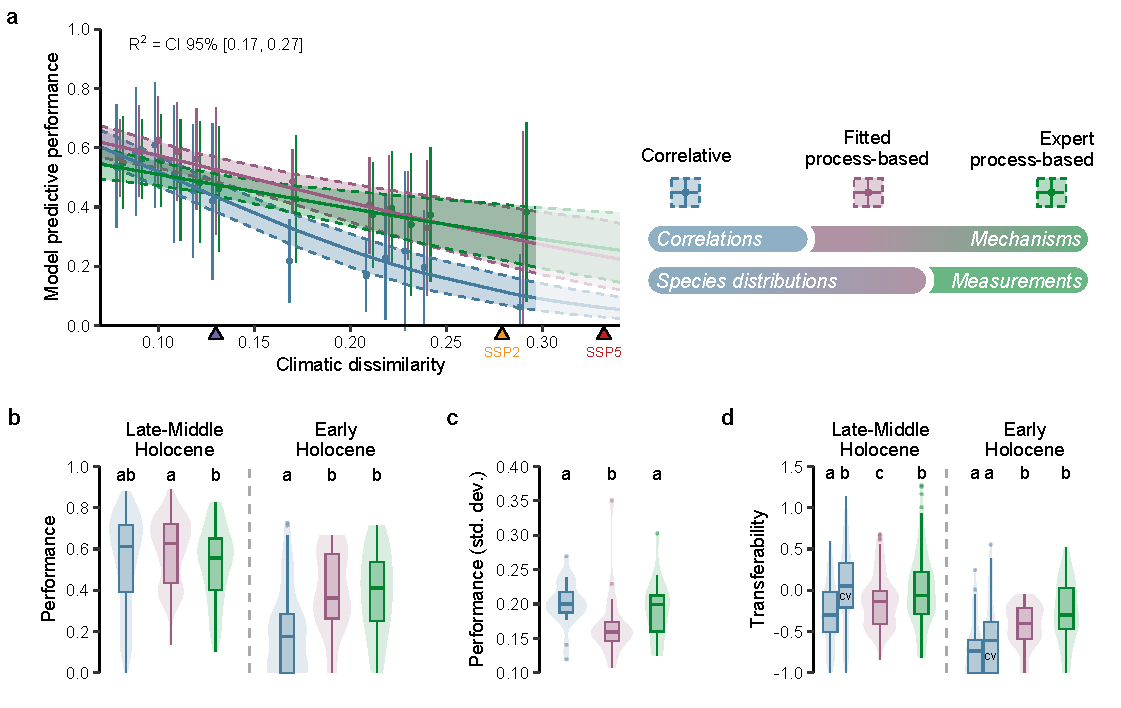
\includegraphics[scale=0.9]{past_performance-1.pdf}
%emw13Jan -- can you add the SSP labels to triangles on Fig a? 
\caption{\textbf{Performance of correlative models, fitted process-based models (inverse calibration using occurrence data) and expert process-based models (classical calibration) against Holocene paleoecogical evidence (fossil pollen) for 4 tree genera (\emph{Abies}, \emph{Fagus}, \emph{Quercus} deciduous and \emph{Quercus} evergreen).} \textbf{(a)} Bayesian beta regression of model predictive performance (Sørensen index) against climatic dissimilarity relative to 1901-2000 (1-Sørensen similarity between climatic hypervolumes). Shaded areas represent 2.5\% and 97.5\% quantiles of the posterior predictive distribution. Points represent the average model performance (and lines the standard deviation) grouped by similar level of climatic dissimilarity . Blue triangle on x-axis indicates the limit between Early Holocene (before 8200BP) and Late-Middle Holocene (after 8200BP). Yellow and red triangles indicate the expected level of climatic dissimilarity in 2060 for SSP245 and SSP585 scenarios. Panel \textbf{(b)} shows the difference of transferability (relative change in model performance between projected period and calibration period) across models. "CV" stands for "cross-validation", when correlative extrapolation errors (in calibration period) were assessed using a block cross-validation method. Panels \textbf{(c)} and \textbf{(d)} show the difference in performance (Sørensen index) and variability in performance (standard deviation of Sørensen index) across models. The grouping letters represent the multiple comparisons with pairwise Conover-Iman tests. }\label{past_performance}
\end{figure}

\item \emph{Can model performance in the past give a hint of their performance in the future?}\par
%emw13Jan -- below is great!
\item Comparing climate dissimilarity to present of scenarios SP245 and SSP585 to that of the last 12 kyr, we  could assess that the predictions of PBMs, either fitted or expert, should be more reliable up to 2060 according to the scenario SSP245 than predictions of CSDMs (\hyperref[past_performance]{Fig. 3a}). However, as soon as 2060, the level of climate dissimilarity predicted by the scenario SSP585 will exceed the range investigated in this study
\item Although hindcast exercices allow evaluating models in very different conditions from those used for their calibration, they do not guarantee their validity in the future. They only provide an evaluation of model consistency with some observations, which does not demonstrate that the model accounts for all processes that could constrain future species distribution \cite{Oreskes1994}. Nevertheless, our study provides a new  objective assessment of species distribution models, strengthening conclusions on climate changes impacts and uncertainties. Acknowledge these uncertainties is as important as to make the predictions themselves \cite{Beale2012} and contributes to the public trust in scientists \cite{Berkhout2010}. Despite different future projections among global climate models (Extended Data Fig. 2), the rate of anthropogenic climate change and the increased probability of occurrence of novel climates (\cite{Williams2007} and \hyperref[climatic_dissimilarity]{Fig. 1}) are challenging the reliability of both CSDMs and PBMs especially when they are intended to be used in more complex models such as biosphere-atmosphere models and by natural resource managers and policy makers to guide management plans and policies.
\item The scarcity and strong uncertainties of pollen data prevented us from assessing model performance prior 11.5kyr BP although our simulations started at 12kyr BP, which could have covered a wider range of conditions since climate dissimilarity sharply increases and doubles from 11.5 to 12 kyr BP. Nevertheless, the accuracy of the starting point of the simulations at 12kyr BP plays a major role in the evaluation of models performance across the Holocene (Extended Data Fig. XX).  From 11.5kyr BP onwards, climatic dissimilarity varies between 0.29 and 0.08, a level equivalent to what we might experience in the first half of the 21st century (\hyperref[climatic_dissimilarity]{Fig. 1}). We can assess that predictions of PBMs, either fitted or expert, should be more reliable at least up to 2060 according to the scenario SSP245 (\hyperref[past_performance]{Fig. 3a}) and 2050 according to SSP585. However, future climatic conditions will shift in a different direction from what happened during the late Pleistocene and early Holocene (Extended Data Fig. 3), challenging us to make a solid quantification of models projections uncertainty and opening up new avenues for model evaluation improvement. Moreover, tree colonization dynamics will likely be very different in the future: it will not only occur from few refugia but wider conitnuous ranges, and direct anthropogenic factors, such as sylvicultural practices and assisted species migration, might also shape the composition of forests (refs). Nevertheless, our results still serve as an important step towards an assessment of model transferability and prediction uncertainties, not solely based on the model's own prediction dispersion. 

\item \emph{Scaling-up process-based models}\par
\item Although they yield no significantly different performance, fitted PBMs showed an intermediate behaviour between CSDMs and expert PBMs. In Late-Middle Holocene, their performance is equivalent to CSDMs (pairwise Conover-Iman test, $P=0.084$, \hyperref[past_performance]{Fig. 3c}), mostly because both types of models use the same data for their calibration, i.e species present distribution, and the fact that climate conditions did not change drastically along this period compared to present (\hyperref[climatic_dissimilarity]{Fig. 1}).  
\item Fitted PBMs bring together the strengths from both CSDMs and expert PBMs approaches by describing causal relationships between environmental conditions and species performance (i.e., from PBM approaches) and precise estimates of parameter values (from CSDM approaches). The differences between expert and fitted PBMs in the Middle-Late Holocene pinpoint some issues in expert parameterisation that requires to combine various methods to cope with both the scarcity of data for each ecophysiological process modelled and sometimes non-measurable parameters (e.g. \citep{DeCaceres2023}).  Some parameters in these relations can be measured directly, and exhibit little variability across a species range (e.g. water potential leading to 50\% of vessels embolism). However, the measurement of parameters in controlled conditions does not necessarily guarantee their external validity \emph{in natura} \cite{Asse2020} where much more factors, not represented in laboratory conditions, can also affect the process modelled (but see \cite{Satake2013}). Other parameters are either highly variable because of local adaptation over long period,  difficult-to-measure or so far unmeasurable (e.g. bud dormancy break date). Therefore, expert PBMs can suffer from uncertainties entailed in the measurements of some of their parameters, and from spurious data specific to few locations which do not represent sufficiently well all the conditions the species can experience all over its range. For all these reasons, inverse calibration can provide a valuable opportunity to estimate the values of PBMs parameters especially difficult to estimate otherwise \cite{Evans2016}. However, inverse calibration using only occurrence data could lead to a misrepresentation of true processes \cite{VanderMeersch2023}, and is only a first step towards a better parametrization of PBMs. Given ongoing improvements to computational methods and newly available observations at a global scale (such as remote sensing LiDAR data), there is an avenue for the extensive use of process-based models to provide both realistic and reliable projections in future climates.

\item \emph{Conclusion?}\par
% CSDMs can teach us process-based model-building strategies that allow for the propagation of errors, and allow to separate uncertainty sources within model (imprecise parameters, input data, ...) ?
% Hybrid approach: "\emph{Interest to balance biological realism and flexibility in model building with limited knowledge}" (IPBES, chapter 4) => citation à rajouter peut-être qq part
% idea in Evans 2012: forecast need to be realistic and need to be reliable in novel conditions \cite{Evans2012} (two conditions) + In climatological research, forecasting is done using process-based models! 
\item The unique multi-model comparison across the Holocene we provide here suggests that our understanding of biological mechanisms embedded into process-based models represent a real advantage as compared to empirical relations used in CSDMs to increase projections reliability in the upcoming decades. However, data availability places limits on how these models can be parameterized, and could explain the difficulty to use them more widely for global impact studies. Fitted PBMs may overcome this problem by using more data at a larger geographical scale, while keeping the predictive strength of causal relationships.
\end{itemize}

\backmatter

\section*{Data and code availability}

Simulation outputs, together with the code to reproduce the analysis and figures in this study, are available on GitHub at \url{https://github.com/vvandermeersch/past_robustness}.

\section*{Acknowledgments}

We acknowledge the support and computing resources of GenOuest and TGCC-CEA. V.V. was supported by a GAIA doctoral school PhD Fellowship.

\section*{Ethics declarations}

The authors declare no competing interests.

%%===========================================================================================%%
%% If you are submitting to one of the Nature Portfolio journals, using the eJP submission   %%
%% system, please include the references within the manuscript file itself. You may do this  %%
%% by copying the reference list from your .bbl file, paste it into the main manuscript .tex %%
%% file, and delete the associated \verb+\bibliography+ commands.                            %%
%%===========================================================================================%%

\bibliography{robustness_bibliography}% common bib file
%% if required, the content of .bbl file can be included here once bbl is generated
%%\input sn-article.bbl


%%Online only Methods should be presented in a separate section after the end of the main text
%% and reference list

\section{Online methods}\label{methods}

\subsection{Correlative and process-based models}\label{models}

Two process-based models were used in this study. 
PHENOFIT simulates the fitness of an average adult tree \cite{Chuine2001}. It estimates fitness components (survival and reproductive success) by simulating the precise phenology (dates of leaf unfolding, flowering, fruit maturation, leaf senescence) and damages caused by abiotic stress (frost, drought) which effects depend on their occurrence relatively to the development stages of the different organs. It has been used for several North American and European species \cite{Morin2007, Saltre2013, Duputie2015, Gauzere2020}. The model has \textappr30 parameters. 
CASTANEA simulates carbon and water cycles of an average adult tree by simulating many processes such as photosynthesis, stomatal opening, maintenance and growth respiration, transpiration and carbon allocation  \cite{Dufrene2005}. It has been used to predict carbon and water budgets of several European species \cite{Davi2006, Delpierre2012, Davi2017}. 
The model has \textappr80 parameters. 
Both models require daily meteorological variables and soil characteristics. 
%emw13Jan -- The below needs to be clearer for readers in the main text I think. 
Two versions of both models were employed: one was calibrated with expert knowledge and statistical inference using observations and measurements of the processes modelled (version called \emph{expert}), and a second one calibrated using species distribution data (version called \emph{fitted}, \cite{VanderMeersch2023}).
  
Four well-established correlative models, whose predictive performances have previously been evaluated \cite{Valavi2022}, were used: GLM with lasso regularization, GAM, BRT and down-sampled Random Forest. We chose four uncorrelated climate predictors related to ecological processes to calibrate these models: minimum temperature of the coldest month (representing frost tolerance), total precipitation (representing available water), GDD5 (growing degree days  \textgreater5°C) between April and September (representing available thermal energy for vegetation growth and fruit maturation), water balance between June and July (precipitation-evapotranspiration, representing summer drought tolerance). We also included two soil covariates (pH and Water Holding Capacity).
  
While by construction correlative models directly output species habitat suitability, we used fitness predicted by the model PHENOFIT and net primary production predicted by the model CASTANEA as a proxy of species habitat suitability. 
CSDMs and inverse-calibrated PBMs were calibrated for five species (\textit{Fagus sylvatica} L., \textit{Abies alba} Mill., \textit{Quercus robur} L., \textit{Quercus petraea}  (Matt.) Liebl. and \textit{Quercus ilex} L.) using historical climate (1970-2000) extracted from ERA5-Land hourly dataset \cite{MunozSabater2021}, soil data from EU-SoilHydroGrids \cite{Toth2017} and SoilGrids \cite{Hengl2017} databases and species occurrence data from the dataset assembled in \cite{VanderMeersch2023}, mostly based on EU-Forest inventory data \cite{Mauri2017}. For each CSDM and each species, we run a fivefold environmental cross-validation to estimate model performance (Extended Data Fig. 9). We then used all the available training data to calibrate the models for the hindcasting in order to favour final prediction quality \cite{Roberts2017}. We could not run the same cross-validation method for fitted process-based models because it would have been too computationally expensive. 

Model simulations over the Holocene were run for 30-year periods every 250 years, for the five above mentioned species. Model outputs were averaged over each 30-year period. Note that soil conditions (needed both for correlative and process-based models) were held constant throughout the simulations. Note also that for CASTANEA model, species specific thresholds of net primary production were computed with the CO$_2$ level at the beginning of the Holocene (\textappr240ppm).

\subsection{Late Quaternary climate and vegetation}\label{paleodata}
%emw13Jan -- are there multiple initial conditions (members)? Not critical, I am just wondering. 
We used a monthly paleoclimate simulation dataset \cite{Armstrong2019} generated with the HadCM3B-M2.1 coupled general circulation model, starting from 18.000BP at 0.5\degree~spatial resolution for Europe (Extended Data Fig. 1). It includes both millennial scale climate variability and inter-annual variability. For this work, several variables were specifically produced: mean temperature, average minimum and maximum daily temperatures, precipitation, number of rainy days, cloudiness, and wind speed (Extended Data Fig. 4). We further downscaled temperature and precipitation monthly data to 0.25\degree~resolution, by applying an elevation correction of coarse-scale variables towards the ICE-6G-C elevation level at high resolution \cite{Peltier2015}.  
We then generated daily data for temperatures, precipitation, cloud cover and wind speed from  the monthly data with the weather generator GWGEN \cite{Sommer2017}, for 30-year periods every 250 years. We also simulated daily extra-terrestrial solar radiation with the same orbital forcing conditions used in HadCM3B-M2.1 \cite{Armstrong2019} and then computed daily global radiation taking into account previously generated daily cloud-cover data as implemented in LPJ-LMfire global model \cite{Pfeiffer2013}. Finally, we computed daily potential evapotranspiration following the standard FAO Penman-Monteith method \cite{Allen1998}.  

Fossil pollen records were extracted from the LegacyPollen dataset \cite{Herzschuh2022}. This dataset is mainly based on the Neotoma database \cite{Williams2018}, and provides samples with standardized chronologies and age uncertainties. We removed sites that had marine depositional environments \cite{Maguire2016}, and only kept samples with more than 200 pollen grain counts and age uncertainty of less than 500 years.
Pollen relative abundances were aggregated to consecutive 500-year intervals. If multiple samples from the same site belonged to the same period, we averaged their pollen abundances, weighting by their age uncertainty and temporal distance from the center of the period. Relative pollen abundances were converted to presence/absence using thresholds based on biome reconstructions \cite{Williams1998}: 1\% for \emph{Fagus} and \emph{Abies}, and 2.5\% for \emph{Quercus}. If several sites fell within the same grid cell (0.25\degree), we considered the species as present if there was at least one site where the species could be considered as present. \textit{Fagus} pollen data were used to assess the presence of \textit{Fagus sylvativa} L., sole species of the genus present in Europe. \textit{Abies} pollen data were used to assess the presence of \textit{Abies alba} Mill., most abundant and widespread fir species present in Europe. When possible, deciduous and evergreen \textit{Quercus} pollen were distinguished based on Neotoma data. Some \textit{Quercus} pollen remain undetermined beyond the generic level, either because discrimination between evergreen and deciduous oak pollen was impossible or because authors were not specific. They were assigned to two categories, based on the evergreen natural range as defined by Atlas Flora Europeae \cite{AFE2005} and EuroVegMap \cite{EVM2003}: pollen outside range were considered as deciduous only occurrences, whereas pollen inside range were considered as both evergreen and deciduous occurrences. Deciduous \textit{Quercus} pollen data were used to assess the presence of \textit{Quercus} \textit{petraea}  (Matt.) Liebl., and \textit{Quercus robur} L., the two most abundant and widespread deciduous oak species in Europe. Evergreen \textit{Quercus} pollen data were used to assess the presence of \textit{Quercus ilex} L., the most abundant and widespread evergreen oak species in Europe.

\subsection{Tree migration}\label{migration}

Models used in this study predict species potential distribution based solely on climatic and soil conditions. To compare model predictions to pollen paleorecords, species migration needs to be simulated as well. To implement migration in the simulations, we run a  cellular automaton \cite{Engler2012} which has proven to be as accurate as more complex approaches \cite{Zurell2016}. We modified the initial version of this dispersal model in order to use both short- and long-distance dispersal kernels. We used species-specific fat-tailed kernels \cite{Zani2022} at a 500 m resolution, and assumed that trees can disperse once a year (Extended Data Fig. 8). Model outputs were assigned to two classes using specific optimal thresholds maximizing model performance in the historical climate: (i) cells where the model output was under the specific threshold were assigned a zero suitability (species cannot survived), and (ii) cells where the  model output was above the threshold, the suitability was rescaled between 0 and 1 (species can migrate). We considered the deciduous \emph{Quercus} suitability as the maximum suitability between \emph{Q. robur} and \emph{Q. petraea}. Migration simulations started from 12000 BP (or 11750 BP when a model simulates no presence at 12000 BP). Note that starting at 11750 BP or 12000 BP does not change our results (Extended Data Fig. 11).

\subsection{Models performance}\label{skill}

We used the Sørensen's similarity index to measure the hindcast performance of the models, based on the confusion matrix. This discrimination measure has been shown to provide adequate estimations of model discrimination capacity,  not biased by species prevalence or an inflated number of true negative predictions \cite{Leroy2018}. We compared the area potentially occupied (not taking migration into account) and occupied (taking migration into account) by the species to the presence/absence data extracted from the LegacyPollen dataset every 500-year interval.

In order to quantify the climatic differences between the calibration conditions (historical climate) and hindcasting conditions (Holocene climate), we computed two different metrics (Extended Data Fig. 2).
We computed the \emph{climate novelty} as in \cite{Burke2019}, i.e. the minimum Mahalanobis distance (which accounts for covariance among variables) computed with vectors of three-month means temperature and three-month sums of precipitation, between each cell at the different time points during the Holocene period and all the cells of the historical climate (the CRU TS v. 4.07 gridded dataset \citep{Harris2020}). 
The \emph{climatic dissimilarity} was calculated as the Sørensen dissimilarity between climatic hypervolumes (a metric of overlap in multidimensional space). We first generated for each period (500-year interval during the Holocene + historical climate) a set of 20 bootstrapped hypervolumes, using R package \emph{hypervolume} \cite{Blonder2018}. Hypervolumes were computed with a Gaussian kernel density estimation method based upon the first three principal component axis from three-month means temperature and three-month sums of precipitation. We then computed overlap statistics (mean and standard deviation of Sørensen index) between the bootstrapped hypervolumes at each type points of the Holocene and the bootstrapped hypervolumes in the historical climate (i.e. 20x20 overlaps).

We computed these climatic metrics for past conditions and for future conditions (30 climate models and 2 scenarios from NEX-GDDP-CMIP6 dataset \citep{Thrasher2022}). Both paleoclimate and future climate data were uniformized with the CRU dataset to maximize comparability among paleoclimate and future climate novelties. The difference (for three-month temperature average) and the ratio (for three-month precipitation sum) between the observations (from 1901 to 2000) and simulations (1901-1950 for HadCM3B, 1951-2000 for CMIP6 projections) were calculated and applied to the whole modeled time period, assuming that the bias was constant.  

Finally, we estimated the effects of past climate novelty (Sørensen's climatic dissimilarity) on model performance (Sørensen index) with a Bayesian ordered beta regression, considering the different types of models (correlative, fitted process-based and expert process-based), using the R package \emph{ordbetareg} \cite{Kubinec2023} and RStan \cite{SDT2023}.
Compared to a  standard beta regression model, this model allows for observations at the bounds (i.e. Sørensen index = 0 or = 1). We took into account the standard deviation of Sørensen's climatic dissimilarity (computed with sets of bootstrapped hypervolumes, see above) as a predictor measurement error.

\end{document}
